\documentclass[oneside,letterpaper]{scrartcl}

% Used Packages
\usepackage[utf8]{inputenc}
\usepackage[english]{babel}
\usepackage{amsmath,amssymb}
\usepackage{graphicx}
\usepackage{hyperref}
\usepackage[]{tocbibind}
\usepackage{wrapfig}
\usepackage{blindtext}

\parindent 0pt

% Commands
\newcommand{\PN}{LTOS}
\def\myscale{0.55}

% Title details
\author{Markus Rose}
\title{\PN\ Quick Guide}
\date{\today}



\begin{document}
\maketitle

\tableofcontents

%==========
\section{About}
\PN\ is a program for localization and detection and tracking of single particles in two-dimensional greyscale TIFF images and videos.

%==========
\section{Installation}

\PN\ is available at \url{https://github.com/MarkusRose/ParticleTracker} under the GPL. It requires a python interpreter, as well as some additional packages provided below. It can be run from the command line, or with a GUI.

\subsection{Getting Python}

\PN\ is written in Python 3.6. The distribution that was used during development and testing is 
Anaconda Python 3 (\url{https://www.anaconda.com/}).


\subsection{Required Packages}

\begin{itemize}
\item numpy
\item scipy
\item pandas
\item matplotlib
\item tkinter
\end{itemize}


\subsection{Running \PN}

\begin{verbatim} python main.py \end{verbatim}

%=================
\section{Using \PN}\parindent 0pt

\subsection{The Graphical User Interface}

\subsubsection{The Main Window}
\begin{wrapfigure}{r}{0.3\textwidth}
\centering
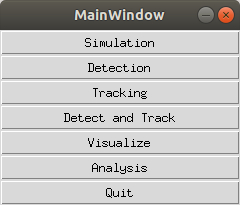
\includegraphics[scale=\myscale]{Figures/MainGUI.jpg}
\caption{Main Menu}
\end{wrapfigure}
\blindtext

\subsubsection{The Detection Menu}
Well
\begin{wrapfigure}{r}{0.5\textwidth}
\centering
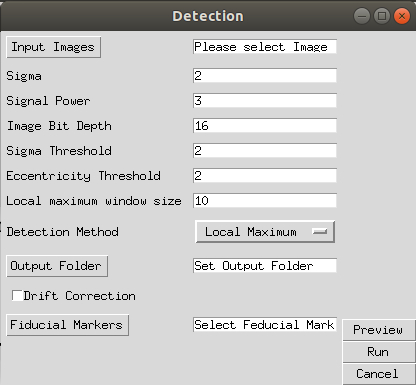
\includegraphics[scale=\myscale]{Figures/DetectionGUI.jpg}
\caption{Detection Menu}
\end{wrapfigure}
\Blindtext

\subsubsection{The Tracking Menu}
\begin{wrapfigure}{r}{0.6\textwidth}
\centering
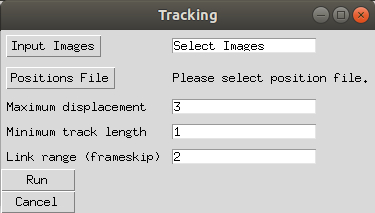
\includegraphics[scale=\myscale]{Figures/TrackingGUI.jpg}
\caption{Tracking Menu}
\end{wrapfigure}
\blindtext

\subsubsection{Detect and Track in one Window}
\begin{wrapfigure}{r}{0.6\textwidth}
\centering
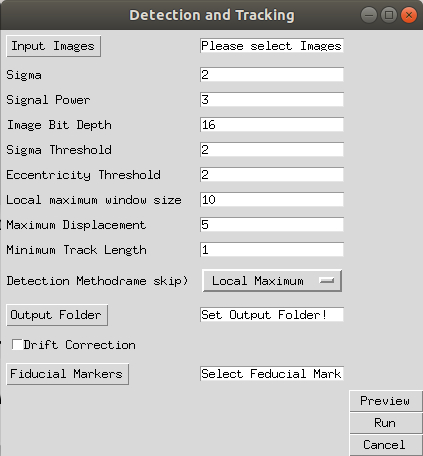
\includegraphics[scale=\myscale]{Figures/DetandTrackGUI.jpg}
\caption{Detect and Track Menu}
\end{wrapfigure}
\blindtext

\subsubsection{Visualization of Images, Detections and Tracks}
\begin{wrapfigure}{r}{0.6\textwidth}
\centering
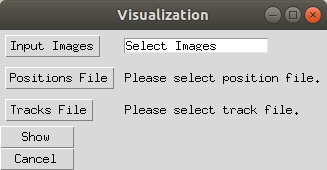
\includegraphics[scale=\myscale]{Figures/VisualizationGUI.jpg}
\caption{Visualization Menu}
\end{wrapfigure}
\blindtext

\subsubsection{Simulation Window}
\begin{wrapfigure}{r}{0.6\textwidth}
\centering
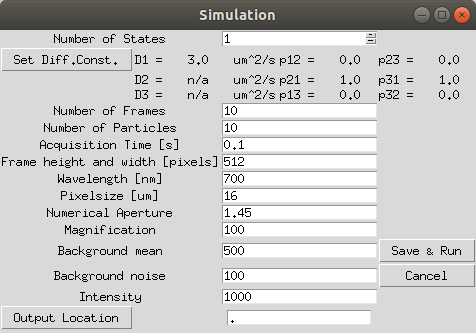
\includegraphics[scale=\myscale]{Figures/SimulationGUI.jpg}
\caption{Simulation Menu}
\end{wrapfigure}
\blindtext

\subsubsection{Analysis Tools for obtained Tracks}
\begin{wrapfigure}{r}{0.6\textwidth}
\centering
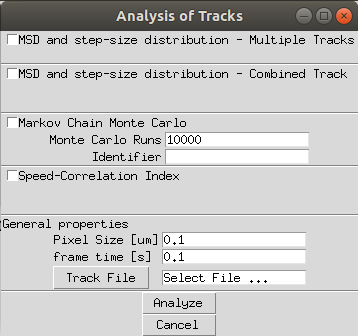
\includegraphics[scale=\myscale]{Figures/AnalysisGUI.jpg}
\caption{Analysis Menu}
\end{wrapfigure}
\blindtext

\subsection{Working from Command Line}

%=================
\section{Program Output}

\bibliographystyle{ieeetr}
\bibliography{biblio}

\end{document}
